\section{Variables for VBF BDT} \label{app:vbf-variables}

The full list of variables considered for the BDT used to define the VBF-enriched signal region is as follows:

\textbf{VBF-targeted:}

$\Delta \eta_{jj}$, $m_{jj}$, $n_{jet}$, $p_{T, \gamma\gamma}/m_{\gamma\gamma}$, $p_{T,jj\bb}$, $p_{T,jjbb}/p_{T,\bb}$\footnote{In these variables $jj$ refers to the VBF-candidate jets, while $\bb$ refers to the $H\rightarrow \bb$ jets}

\textbf{$\gamma \gamma$-suppressing:}

\myybb, $\Delta R_{\gamma\gamma}$, $\Delta R_{\bb}$, $\Delta R_{\gamma \gamma,\bb}$, and the best b-tagging WP for the $H\rightarrow \bb$ jets

\textbf{$ttH$-suppressing:}

$H_{T}$, $m_{jj,b1}$, $m_{jj,b2}$, $m_{jj,W1}$, $m_{jj,W2}$. Event shape variables \cite{STDM-2011-33} - aplanority, aplanarity, sphericity, spherocity, sphericityT, planarity, circularity, planarFlow

The pruning procedure described in Section \ref{ssec:vbf-event-selection} removed the following variables:

\begin{center}
  \begin{table}[h]
	  \begin{tabularx}{\textwidth}{Y|Y}
	    \hline
	    Pruning Step & Variables Removed  \\
	    \hline
      Variables with Pearson correlation $r_{xy} > 0.85$  &  $p_{T,jj\bb}$, $p_{T, \gamma\gamma}/m_{\gamma\gamma}$, sphericity, spherocity, planarity, circularity \\
      \hline
	    Variables with $\sum\limits_{p=0}^{3} r_{x,p} < 1.0$ for BDT-class probabilities, $p$ &  $n_{jet}$, $p_{T,jjbb}/p_{T,\bb}$, $\Delta R_{\gamma \gamma,\bb}$, aplanarity, $H_{T}$, $m_{jj,b1}$, $m_{jj,b2}$, $m_{jj,W1}$ \\
	    \hline
    \end{tabularx}
  \end{table}
\end{center}


% TODO: once variables in framework, switch these to official plots

Distributions for all considered variables are shown in Figure \ref{fig:vbf-focused-variables}, in which each histogram has been normalized such that its integral is unity. Preselection and a 4-jet requirement has been applied.

\begin{figure}[htbp]
    \centering
    \subfloat{
      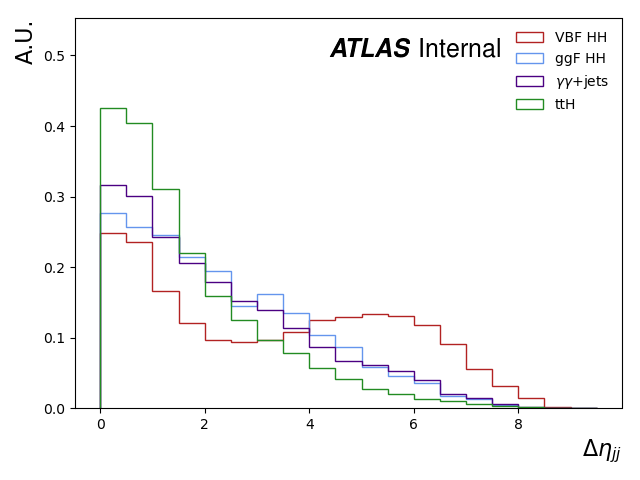
\includegraphics[width=0.48\textwidth]{appendices/vbf-variables/jj_deta.png}
    }
    \subfloat{
      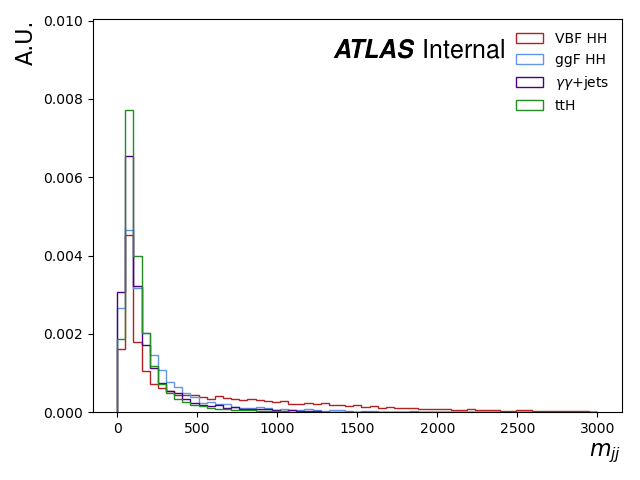
\includegraphics[width= 0.48\textwidth]{appendices/vbf-variables/mjj.png}
    }

    \subfloat{
        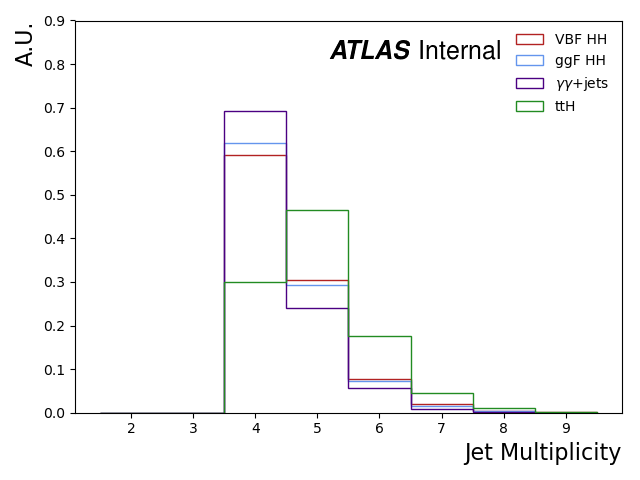
\includegraphics[width=0.48\textwidth]{appendices/vbf-variables/n_jet.png}
      }
      \subfloat{
        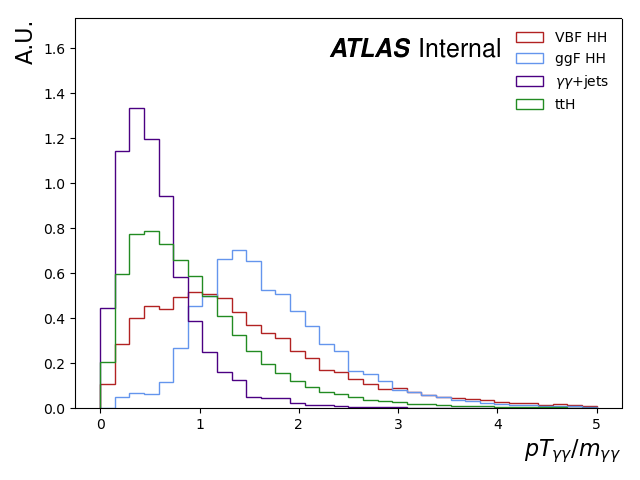
\includegraphics[width= 0.48\textwidth]{appendices/vbf-variables/ptyy_myy_ratio.png}
      }

    \subfloat{
        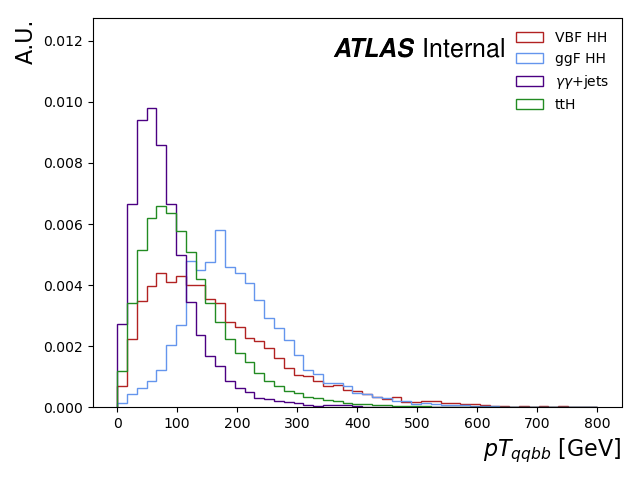
\includegraphics[width= 0.48\textwidth]{appendices/vbf-variables/pt_qqbb.png}
    }    
    \subfloat{
        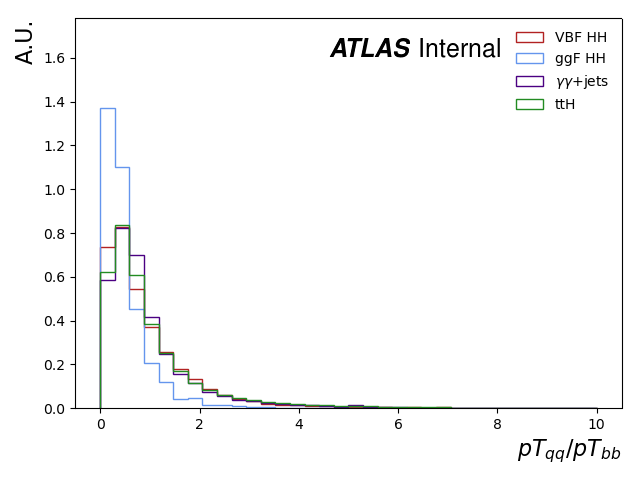
\includegraphics[width= 0.48\textwidth]{appendices/vbf-variables/pt_qq_bb_ratio.png}
    }  

    \caption{Distributions of variables for targeting VBF HH production considered for use the VBF BDT}
    \label{fig:vbf-focused-variables}
\end{figure}


\begin{figure}[htbp]
    \centering
    \subfloat{
      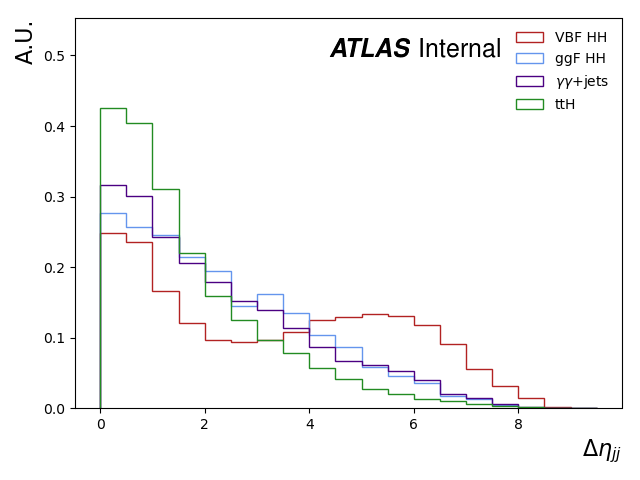
\includegraphics[width=0.48\textwidth]{appendices/vbf-variables/jj_deta.png}
    }
    \subfloat{
      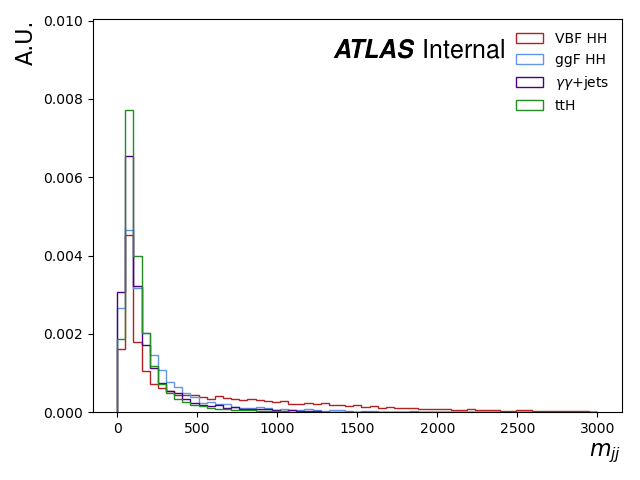
\includegraphics[width= 0.48\textwidth]{appendices/vbf-variables/mjj.png}
    }

    \subfloat{
        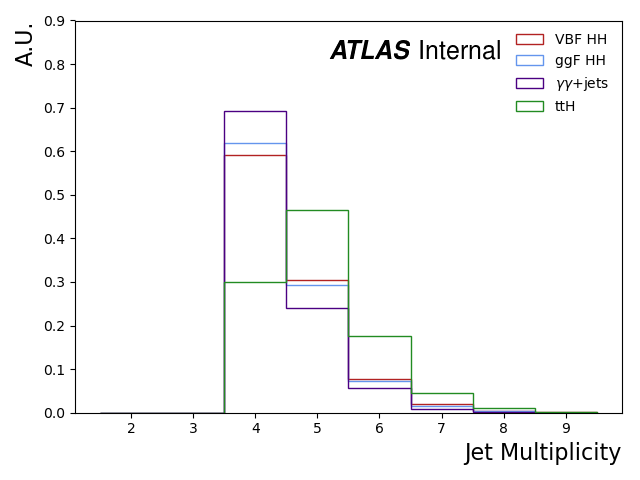
\includegraphics[width=0.48\textwidth]{appendices/vbf-variables/n_jet.png}
      }
      \subfloat{
        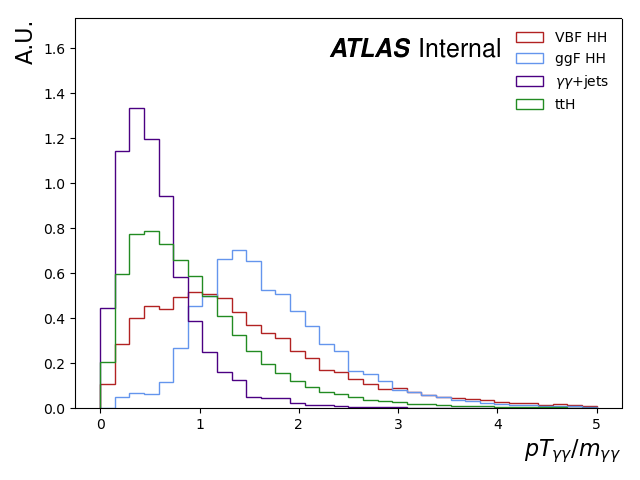
\includegraphics[width= 0.48\textwidth]{appendices/vbf-variables/ptyy_myy_ratio.png}
      }

    \subfloat{
        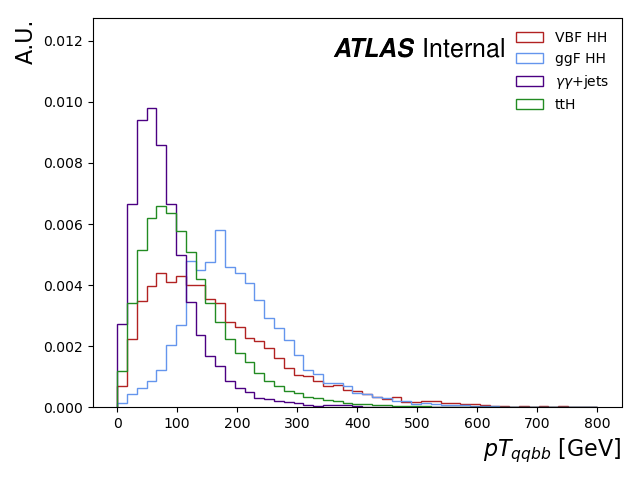
\includegraphics[width= 0.48\textwidth]{appendices/vbf-variables/pt_qqbb.png}
    }    
    \subfloat{
        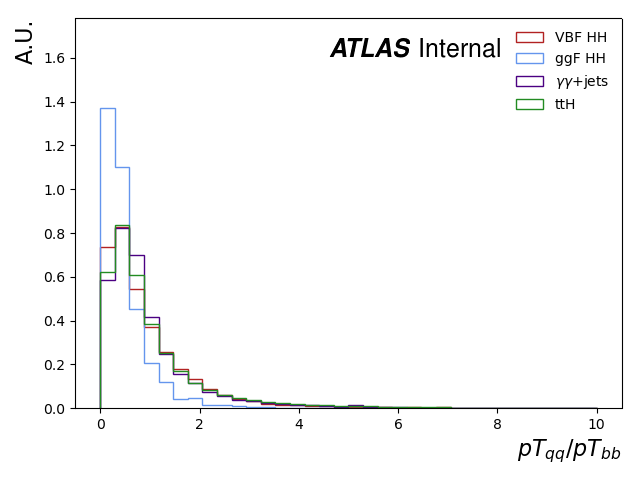
\includegraphics[width= 0.48\textwidth]{appendices/vbf-variables/pt_qq_bb_ratio.png}
    }  

    \caption{Distributions of variables for targeting VBF HH production considered for use the VBF BDT}
    \label{fig:vbf-focused-variables}
\end{figure}

\begin{figure}[htbp]
    \centering
    \subfloat{
      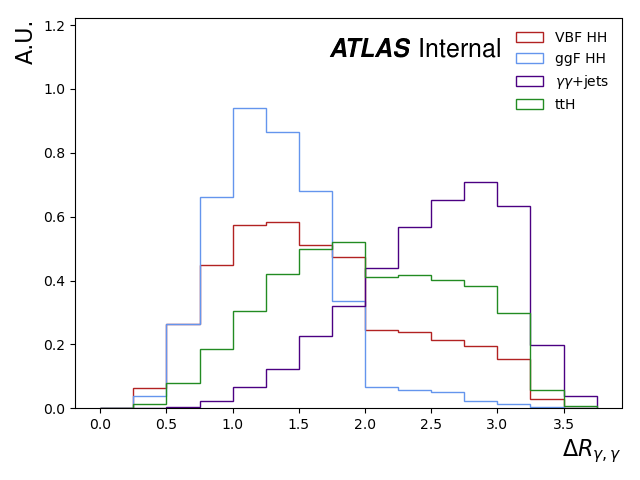
\includegraphics[width=0.48\textwidth]{appendices/vbf-variables/dR_yy.png}
    }
    \subfloat{
      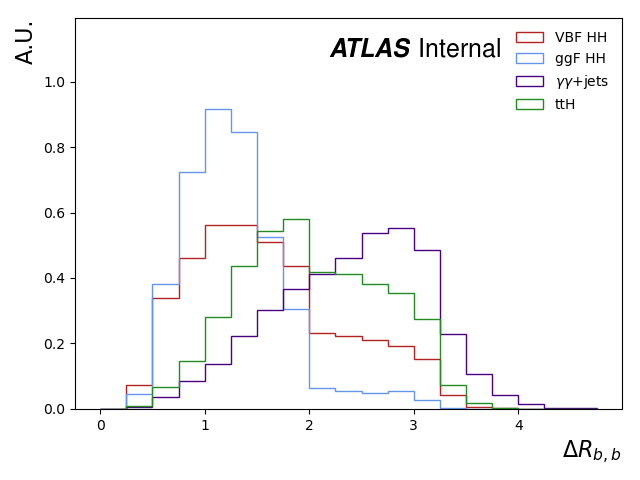
\includegraphics[width= 0.48\textwidth]{appendices/vbf-variables/dR_bb.png}
    }

    \subfloat{
        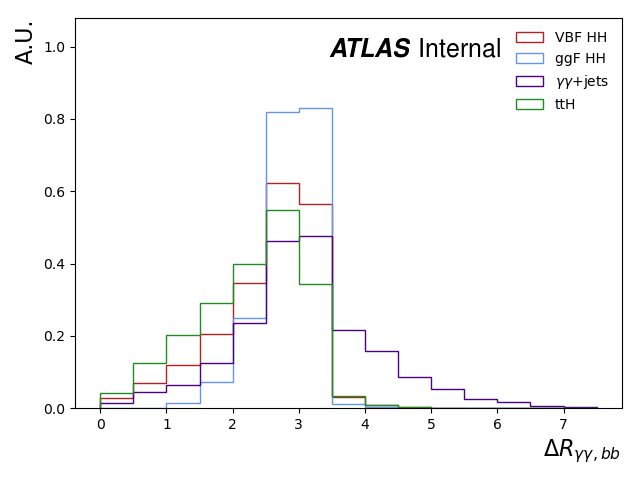
\includegraphics[width=0.48\textwidth]{appendices/vbf-variables/dR_yybb.png}
      }
      \subfloat{
        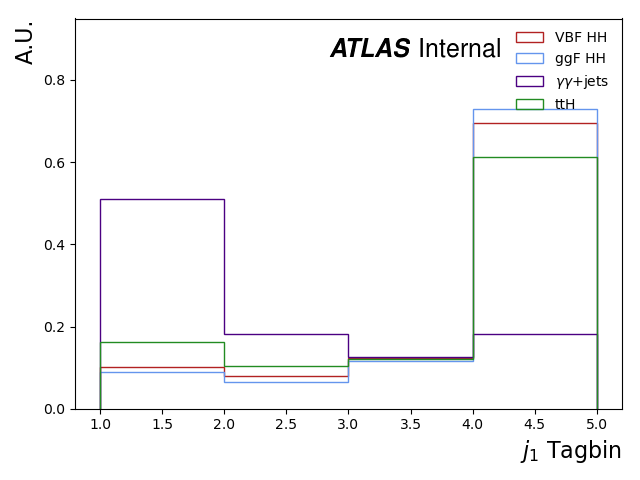
\includegraphics[width= 0.48\textwidth]{appendices/vbf-variables/j1_tagbin.png}
      }

    \subfloat{
        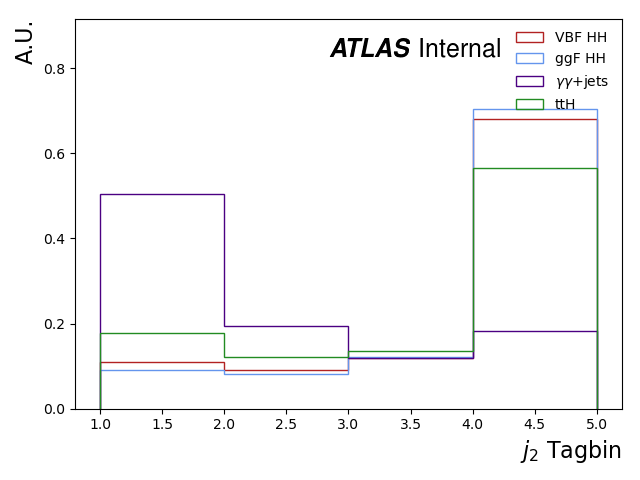
\includegraphics[width= 0.48\textwidth]{appendices/vbf-variables/j2_tagbin.png}
    }    

    \caption{Distributions of variables for suppressing the $\gamma\gamma$ background considered for use the VBF BDT}
    \label{fig:yy-focused-variables}
\end{figure}

% TODO: add w-mass variables

\begin{figure}[htbp]
    \centering
    \subfloat{
      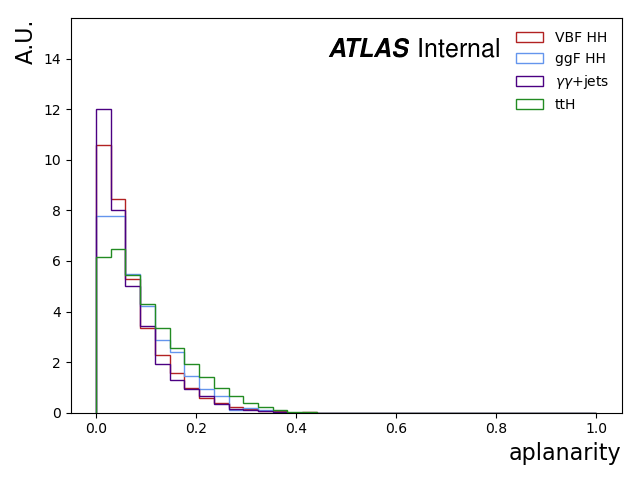
\includegraphics[width=0.48\textwidth]{appendices/vbf-variables/aplanority.png}
    }
    \subfloat{
      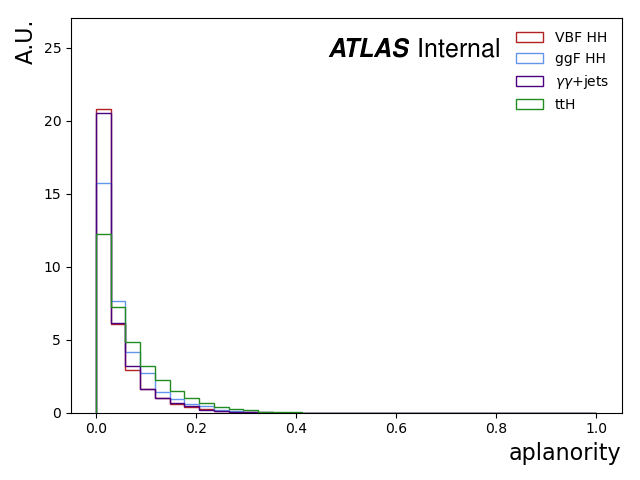
\includegraphics[width= 0.48\textwidth]{appendices/vbf-variables/aplanarity.png}
    }

    \subfloat{
        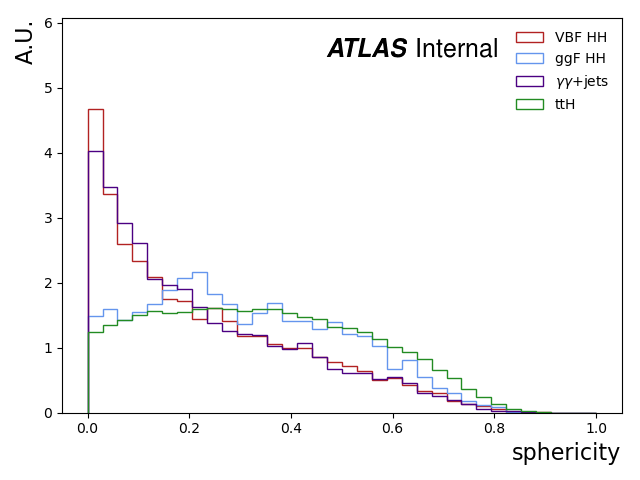
\includegraphics[width=0.48\textwidth]{appendices/vbf-variables/sphericity.png}
      }
      \subfloat{
        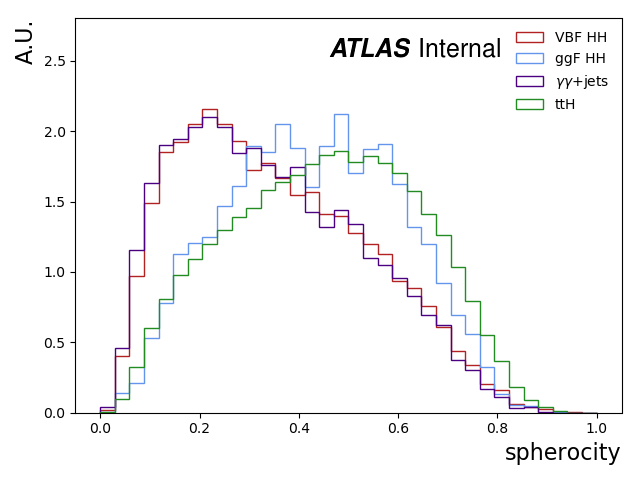
\includegraphics[width= 0.48\textwidth]{appendices/vbf-variables/spherocity.png}
      }

    \subfloat{
        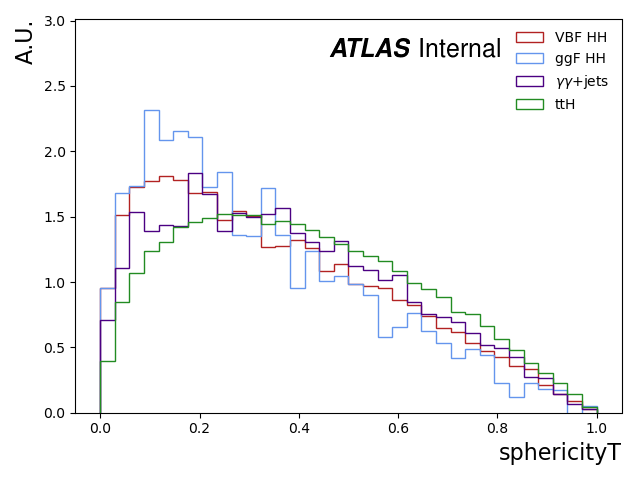
\includegraphics[width= 0.48\textwidth]{appendices/vbf-variables/sphericityT.png}
    }   
    \subfloat{
        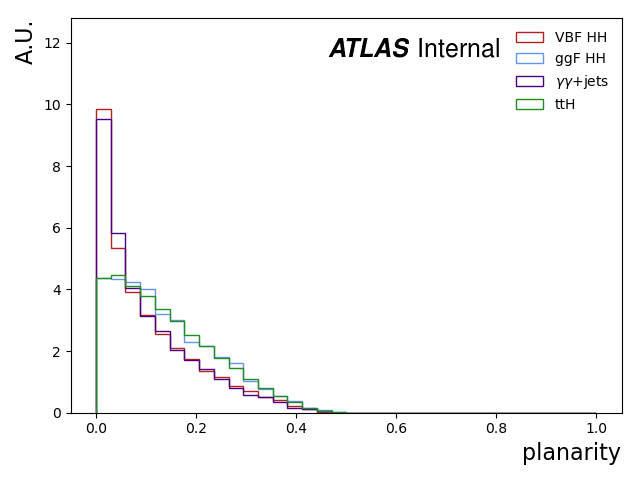
\includegraphics[width= 0.48\textwidth]{appendices/vbf-variables/planarity.png}
    }  

     

    \caption{Distributions of event shape for suppressing the $ttH$ background considered for use the VBF BDT}
    \label{fig:yy-focused-variables}
\end{figure}
\begin{figure}[htbp]\ContinuedFloat
    \subfloat{
        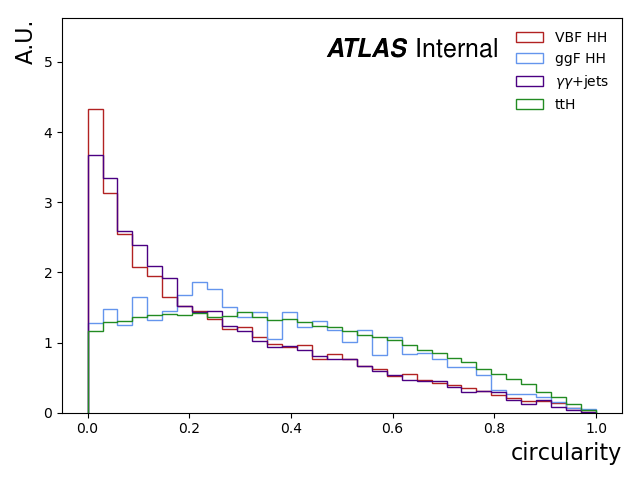
\includegraphics[width= 0.48\textwidth]{appendices/vbf-variables/circularity.png}
    }  
    \subfloat{
        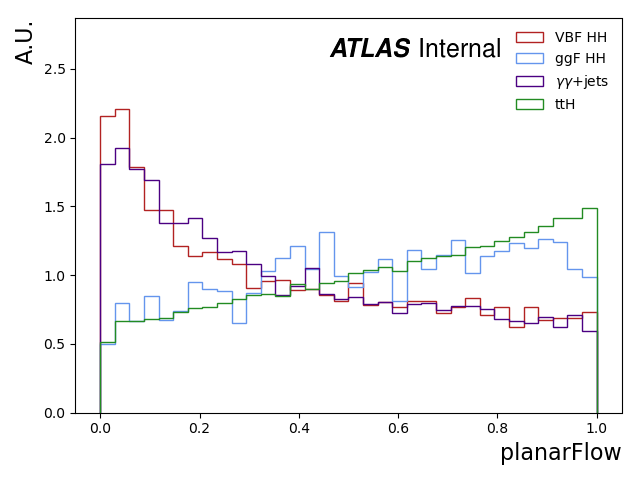
\includegraphics[width= 0.48\textwidth]{appendices/vbf-variables/planarFlow.png}
    }       
        
    \caption{Distributions of event shape for suppressing the $ttH$ background considered for use the VBF BDT}
    \label{fig:yy-focused-variables}
\end{figure}
